\chapter[Cronograma]{Cronograma}

\graphicspath{{figuras/}}

\begin{figure}[!htb]
 \centering
 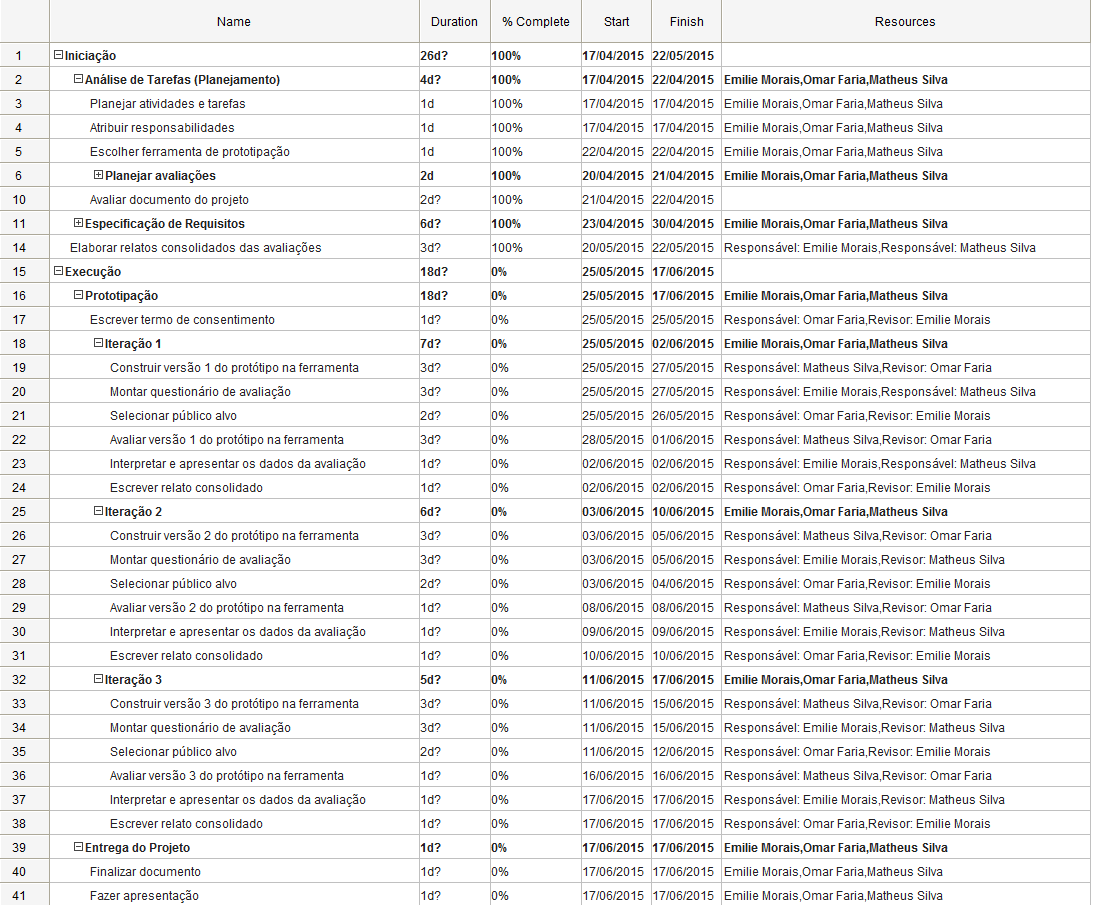
\includegraphics[width = 17.5cm, height = 15cm]{cronograma.png}
 \caption{Cronograma de Atividades}
 \label{Rotulo}

\end{figure}

\subsection{Planejamento da Avaliação}

As avaliações serão feitas permeando todas as fases do processo, assim como sugere o
Modelo Estrela. Serão escolhidos usuários-chave para uso de protótipos do aplicativo em
situações pré-determinadas. Na fase de iniciação do projeto, os usuários avaliarão protótipos
de papel, para levantamento de requisitos. Na execução, com protótipos de alta fidelidade, já
refinado, esses usuários responderão a questionários referentes a questões de usabilidade, bem
como serão coletadas informações no momento da avaliação, como reações do usuário
observadas. Os questionários a serem aplicados, bem como as metas a serem atingidas estão
descritos neste documento nas seções \ref{questionarios} e \ref{metas}, respectivamente.